%% ---------------------------------------------------------------------
%% Mathematical Biosciences (Elsevier) -- manuscript source
%% Class : elsarticle, "review" layout (single column, 1.5 spacing)
%% Refs  : numbered, elsarticle-num
%% ---------------------------------------------------------------------
\pdfminorversion=7
\documentclass[review,12pt]{elsarticle}

\usepackage[T1]{fontenc}
\usepackage{lmodern}
\usepackage{graphicx}
\usepackage{multirow}
\usepackage{amsmath,amssymb,amsfonts}
\usepackage{amsthm}
\usepackage{mathrsfs}
\usepackage{booktabs}
\usepackage{url}
\usepackage{lineno}
\usepackage{caption}

%% The "review" option double-spaces the whole document, which pushes the two
%% longest figure captions off the page.  Captions are set small and
%% single-spaced so that no figure has to be shrunk for the review copy.
\DeclareCaptionFont{singlespaced}{\renewcommand{\baselinestretch}{1}\selectfont}
\captionsetup{font={small,singlespaced}}

%% lineno does not number amsmath display environments unless they are wrapped
%% in \linenomath.  Standard patch from the lineno documentation.
\newcommand*\patchAmsMathEnvironmentForLineno[1]{%
  \expandafter\let\csname old#1\expandafter\endcsname\csname #1\endcsname
  \expandafter\let\csname oldend#1\expandafter\endcsname\csname end#1\endcsname
  \renewenvironment{#1}%
    {\linenomath\csname old#1\endcsname}%
    {\csname oldend#1\endcsname\endlinenomath}}%
\newcommand*\patchBothAmsMathEnvironmentsForLineno[1]{%
  \patchAmsMathEnvironmentForLineno{#1}%
  \patchAmsMathEnvironmentForLineno{#1*}}%
\AtBeginDocument{%
  \patchBothAmsMathEnvironmentsForLineno{equation}%
  \patchBothAmsMathEnvironmentsForLineno{align}%
  \patchBothAmsMathEnvironmentsForLineno{flalign}%
  \patchBothAmsMathEnvironmentsForLineno{alignat}%
  \patchBothAmsMathEnvironmentsForLineno{gather}%
  \patchBothAmsMathEnvironmentsForLineno{multline}%
}

\numberwithin{equation}{section}

\theoremstyle{remark}
\newtheorem{remark}{Remark}

\raggedbottom

\newcommand{\ABM}{\mathrm{ABM}}
\newcommand{\HD}{\mathrm{HD}}

\journal{Mathematical Biosciences}

\begin{document}

\linenumbers

\begin{frontmatter}

\title{Overlapping roots: a transmission-tree framework for population-level contact-tracing dynamics}

\author[a,b]{Seyfullah Enes Kotil\corref{cor1}}
\ead{enesseyfullah.kotil@bogazici.edu.tr}
\cortext[cor1]{Corresponding author.}

\affiliation[a]{organization={Department of Molecular Biology and Genetics,
                              Bo\u{g}azi\c{c}i University},
                city={Istanbul},
                country={T\"urkiye}}

\affiliation[b]{organization={School of Medicine, Department of Biophysics,
                              Bah\c{c}e\c{s}ehir University},
                city={Istanbul},
                country={T\"urkiye}}

\begin{abstract}
All contact-tracing models are incomplete, but all must be elegant. The central modeling challenge is to retain enough transmission history to determine tracing losses. We introduce a root-centered framework that preserves the transmission structure needed for contact tracing while remaining interpretable and usable at the population level. Every infectious individual is viewed as the root of a local active genealogy. Aggregating these overlapping views gives population variables that count infectious cases one, two, and more transmission steps downstream. For instantaneous one-step forward tracing, the population-level tracing loss is proportional to the number of infectious cases one step downstream. The resulting open hierarchy of population equations admits tractable finite-depth closures. Early-growth analysis gives simple approximations for epidemic growth and the future infectious activity generated by newly infected cases. In this idealized setting, maximal one-step tracing reverses early growth only when the dimensionless baseline transmission strength satisfies $R<R_*(1)\approx 1.67$. Above this threshold, tracing does not achieve control but can still reduce future infectious activity by approximately 40\% relative to no tracing. Under susceptible depletion, the closures generate complete epidemic trajectories, which we compare with large-population agent-based ensemble averages generated from the same event rules. Developed here in the simplest forward-tracing setting, the framework bridges individually resolved transmission histories and compartmental models and provides a foundation for extensions to backward and bidirectional tracing, repeated tracing rounds, latent periods, and explicit delays.
\end{abstract}

\begin{keyword}
Contact tracing \sep Overlapping roots \sep Transmission genealogy \sep
Moment closure \sep Epidemic model \sep Agent-based model
\end{keyword}

\end{frontmatter}

\section{Introduction}\label{sec1}

In contact tracing, once an infectious case is detected, epidemiologically linked individuals are identified, their infection risk is assessed, and those who may transmit are tested, monitored, quarantined, or isolated. The intervention is straightforward to state but difficult to model mathematically.

The difficulty is that the population-level effect of tracing cannot be determined from compartment counts alone. Under standard well-mixed assumptions, aggregate infection and recovery flows can be expressed in terms of the numbers of susceptible and infectious individuals. Tracing outcomes, however, depend on where detected cases lie within the realized transmission graph. Tracing may proceed from a detected case to its infectees (forward tracing), to its infector (backward tracing), or in both directions (bidirectional tracing). The problem is therefore intrinsically multiscale: population counts describe aggregate epidemic dynamics, whereas the transmission graph determines how the detection of one case affects others.

This is already visible in the simplest comparison. Two epidemics can have the same numbers of susceptible and infectious individuals yet experience different tracing losses. If detected cases in one epidemic have many infectees who remain infectious, forward tracing removes more additional cases than when detected cases have few such infectees. A compartmental model can therefore represent aggregate infection and recovery flows while still lacking the local structure needed to calculate tracing losses.

The mathematical theory of contact tracing spans several decades and includes many modeling approaches \cite{muller2021}. Two broad lines of work provide reference points for the intermediate representation developed here.

Branching-process and named-contact models begin from the approximately tree-like structure of transmission during the early epidemic, when branches are approximately independent and are not constrained by depletion of susceptible individuals. Contact tracing punctures this randomly generated structure: the detection of one case removes other cases according to their genealogical positions, and the central question becomes how the interrupted tree survives and reproduces through successive generations. Because parent and offspring positions are explicit, the distinction between forward and backward tracing arises naturally, while latent periods and tracing delays can be incorporated directly \cite{muller2000,klinkenberg2006,ball2011,ball2015,muller2016,okolie2020,muller2023}. These formulations are particularly powerful for early-phase dynamics. Their primary mathematical object is the transmission genealogy, whereas the finite-population trajectory is generally described at a different level; coupling genealogical structure directly to time-varying population dynamics therefore requires an additional representation or reduction.

Pairwise, message-passing, and related network models make a different choice. They remain within a population-level dynamical system but supplement node counts with states for epidemiologically relevant pairs. The evolution of pairs depends on triples, triples depend on higher-order configurations, and the resulting hierarchy is closed at a selected structural level, making the population model aware of local contact correlations \cite{eames2003,house2010,karrer2010,sharkey2015a,sharkey2015b,pellis2015,wilkinson2017}. This produces a unified population-level description, but infection direction is not automatically the organizing coordinate of a pair state: forward and backward tracing can be represented, yet their distinction must be encoded in the selected states or transitions. More aggregated compartmental models provide another reduction by introducing detected, traced, or treated classes and their transfer terms \cite{hethcote1984,dearazoza2002,hyman2003,hsieh2010}.

A particularly close comparison is the model of Zhang and Britton~\cite{zhang2022}, which bridges an early branching description and population-level dynamics through carefully chosen graph states. Transmission links are labeled according to whether they would be reported, and infectious individuals are organized into to-be-reported components, tracked by the fraction of infectious individuals belonging to components of each size. Distinct components behave independently in the early limit, whereas the main epidemic phase is described by an infinite deterministic system for the component-size distribution. The resulting mathematical object is an infinite component-size hierarchy, truncated at a sufficiently large component size for numerical work.

The present work follows the same broad strategy of translating graph events into population-level equations, but adopts a different graph coordinate. Zhang and Britton organize infectious individuals by to-be-reported component size, a natural coordinate for tracing mechanisms that act on such components. We instead organize the population by directed descendant position relative to overlapping active roots, which is convenient when detection of a root acts directly on its active infectees. The two constructions retain different aspects of the transmission graph in accordance with the intervention being represented.

The construction is as follows. Every currently infectious individual is treated as the root of its own local active genealogy. The same physical individual may therefore appear as a child in its infector's local view, as a grandchild or deeper descendant in an earlier ancestor's view, and simultaneously as the root of its own local view. These local genealogies overlap, but individuals are not duplicated: each infectious case is counted once as a physical individual, and the terms child, grandchild, and deeper descendant specify only its position relative to a selected root. Aggregating these overlapping views across the infectious population yields variables for which genealogy-dependent tracing losses take simple population-level forms. The resulting system does not close with finitely many variables and therefore forms an infinite deterministic genealogical hierarchy.

We develop this hierarchy in the simplest setting of instantaneous one-step forward tracing, which allows the root-relative representation and the tracing dynamics to be presented transparently. We analyze it first in the early-growth regime, where a quasi-steady reduction yields explicit approximations and epidemiological quantities, and then under susceptible depletion, where finite-depth closures generate complete epidemic trajectories that we compare with large-population agent-based ensembles generated from the same event rules. Under maximal one-step tracing, early growth can be reversed only when the dimensionless baseline transmission strength is below a control boundary $R_*(1)\approx1.67$; above this boundary, tracing cannot make the epidemic subcritical, although it still substantially reduces future infectious activity. The framework can in principle be extended to backward and bidirectional tracing, repeated tracing rounds, latent periods, and explicit delays through suitable modifications of the root-relative coordinates and event rules.

\section{The overlapping-roots construction}\label{sec2}

This section builds the population variables that make forward-tracing losses computable, starting from individual events.

\subsection{Model assumptions and tracing mechanism}\label{subsec2.1}

Consider a closed population of fixed size $N$. At time $t$, let $S(t)$ denote the number of susceptible individuals and let $\mathcal A(t)$ denote the set of currently infectious individuals, so that the infectious population count is $I(t)=|\mathcal A(t)|$. Each infectious individual generates infections at rate $\beta S$, where $\beta$ is the per-susceptible transmission rate, giving an aggregate transmission rate $\beta S I$. A newly infected individual leaves the susceptible population, becomes infectious immediately, and is assigned the transmitting individual as its unique parent. The unique-infector assumption makes the realized transmission genealogy a directed forest, with one component for each unrelated initial infectious individual.

Each infectious individual undergoes spontaneous removal, such as recovery, at rate $\gamma$, and case detection at rate $\gamma_c$. We write
\begin{equation}
\Gamma = \gamma + \gamma_c
\label{eq:2.2}
\end{equation}
for the total primary removal rate, where primary removal means removal caused by the individual's own recovery or detection mechanism. When primary removal occurs through detection, each direct infectee of the detected individual who remains infectious is independently traced with probability $p_f$ and, if successfully traced, is removed immediately. A removal caused by tracing does not initiate an additional tracing event. The model therefore describes instantaneous one-step forward tracing with immediate infectiousness, unique parentage, no latent period, no tracing delay, no backward tracing, and no recursive or repeated tracing cascade.

Three mechanisms consequently contribute to the deterministic population balances: transmission, primary removal, and forward-tracing removal. Transmission and primary removal can be represented using the aggregate counts $S$ and $I$. Forward tracing cannot, because its effect depends on which infectious individuals are active direct infectees of a detected case. Table~\ref{tab:notation} collects the notation used throughout.

\begin{table}[htbp]
\centering
\caption{Notation. Root-relative terms specify position with respect to a selected root, not a biological type.}\label{tab:notation}
\begin{tabular}{@{}ll@{}}
\toprule
Symbol & Meaning \\
\midrule
$S$, $I$ & susceptible and infectious population counts \\
$\mathcal A(t)$ & set of infectious individuals; $I=|\mathcal A|$ \\
$\mathcal C_i(t)$ & active children of $i$: direct infectees of $i$ still infectious \\
$D_i^{(k)}(t)$ & active descendants at depth $k$ in the view rooted at $i$; $D_i^{(0)}=1$ \\
$X_i=D_i^{(1)}$ & number of active children of root $i$ \\
$I_r$ & number of infectious roots with exactly $r$ active children \\
$M_k=\sum_i D_i^{(k)}$ & population count of depth-$k$ root--descendant relations; $M_0=I$ \\
$m_k=M_k/I$ & mean active depth-$k$ descendants per infectious root; $m_0=1$ \\
$\beta,\ \gamma,\ \gamma_c$ & transmission, spontaneous-removal, and detection rates \\
$\Gamma=\gamma+\gamma_c$ & total primary-removal rate \\
$p_f$ & probability that an active child of a detected case is traced \\
$\tau=\Gamma t$ & dimensionless time \\
$R=\beta S_0/\Gamma$ & baseline transmission strength \\
$R_S=\beta S/\Gamma$ & susceptibility-adjusted transmission strength \\
$c=(\gamma_c/\Gamma)p_f$ & forward-tracing intensity, $0\leq c\leq1$ \\
\bottomrule
\end{tabular}
\end{table}

\subsection{Overlapping rooted views, and why $M_1$ is the tracing loss}\label{subsec2.2}

We retain the infector--infectee relationships among individuals who remain infectious, a structure we call the active transmission genealogy, and describe it through overlapping rooted views: each infectious individual is treated in turn as a local root, and its active descendants are represented relative to that root. Each rooted view retains only descendant information; the identity of a root's own infector is not part of that view. No information is lost, because the same relationship is recorded as a descendant relation in the rooted view of the infector.

For $i\in\mathcal A(t)$, let $\mathcal C_i(t)$ denote the set of direct infectees of $i$ who remain infectious at time $t$. When $i$ is selected as a local root, the members of $\mathcal C_i(t)$ are its active children; their active children are the active grandchildren of $i$, and the construction continues through progressively deeper generations. The terms root, child, and grandchild specify positions relative to the selected root; they do not denote different biological types. The same physical case may appear as a child in the local view of its infector, as a deeper descendant in the view of an earlier ancestor, and simultaneously as the root of its own local view. These local views overlap, but they do not duplicate physical individuals.

Retaining only the first generation of each rooted view, define the active child count of root $i$ and the corresponding child-count classes by
\begin{equation}
X_i(t) = |\mathcal C_i(t)|, \qquad
I_r(t) = \sum_{i\in\mathcal A(t)} \mathbf 1_{\{X_i(t)=r\}}, \quad r\geq0,
\label{eq:2.3}
\end{equation}
where $\mathbf 1_{\{\cdot\}}$ is the indicator function, so that $I_r$ is the number of infectious roots with exactly $r$ active children and $I=\sum_{r\geq0}I_r$. The total number of active children carried by the infectious population is
\begin{equation}
M_1(t) = \sum_{r\geq0} r I_r(t) = \sum_{i\in\mathcal A(t)} X_i(t).
\label{eq:2.7}
\end{equation}

This single quantity determines the immediate forward-tracing loss. When a root in class $r$ is detected, it has $r$ active children, each independently traced and removed with probability $p_f$. Roots in class $r$ are detected at total rate $\gamma_c I_r$, so each detection produces on average $rp_f$ tracing-induced removals. Summing over classes,
\begin{equation}
\left.\frac{dI}{dt}\right|_{\text{forward}} = -\sum_{r\geq0} \underbrace{\gamma_c I_r}_{\text{detection rate, class }r}\, \underbrace{r p_f}_{\text{expected removed children}} = -\gamma_c p_f M_1.
\label{eq:2.8}
\end{equation}
The genealogy-dependent intervention has thus acquired an exact population-level form, expressed through one aggregate count.

Equation~\eqref{eq:2.8}, however, does not determine which classes the traced individuals are removed from. To calculate the tracing contribution to each $I_r$ equation, we would need the active-child counts of the traced individuals themselves. That information is not contained in the first-generation classes, so the first-generation system determines the total forward-tracing loss but not the resulting changes in the individual classes: it is not closed under forward tracing. A proportional-allocation benchmark that closes the system by assumption, rather than by construction, is recorded in Supplementary Material 1, Section S1.1.

Figure~\ref{fig:fig1} makes both the bookkeeping and this gap concrete. In the forest shown, root $i$ has $D_i^{(1)}=3$ active children, $D_i^{(2)}=2$ active grandchildren, and $D_i^{(3)}=2$ active great-grandchildren, while its child $j$ carries $D_j^{(1)}=2$ and $D_j^{(2)}=2$ in its own view. If $i$ is detected, the expected physical loss is $p_f D_i^{(1)}=3p_f$ infectious individuals. But each traced child also carries its own descendant information: the depth-1 information lost is $p_f\sum_{j\in\mathcal C_i}D_j^{(1)}=p_f D_i^{(2)}=2p_f$, and the depth-2 information lost is $p_f D_i^{(3)}=2p_f$. Every level of this bookkeeping is expressed by the level below it in the same rooted view --- which is exactly the structure the next subsection formalizes.

\begin{figure}[htbp]
\centering
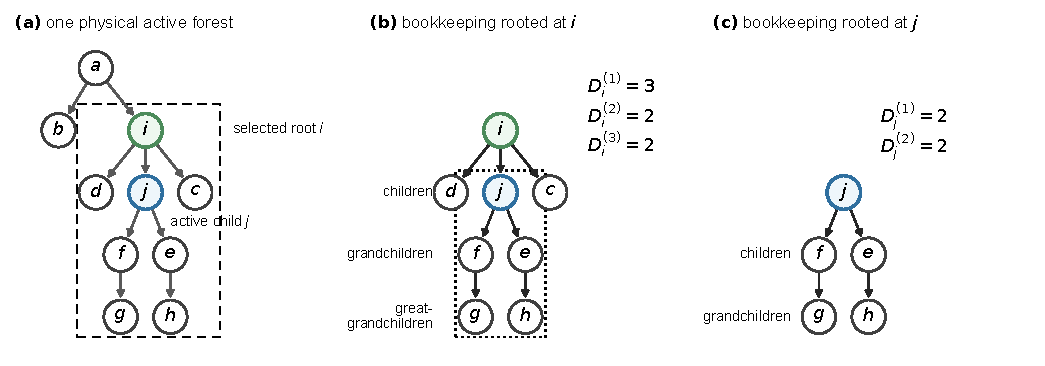
\includegraphics[width=0.96\textwidth]{Fig1.pdf}
\caption{Root-centered bookkeeping in one physical active transmission forest. (a) A single physical active genealogy, with active individual $i$, its active child $j$, and the physical subtree descended from $i$ indicated by the dashed boundary. (b) The same active individuals viewed in coordinates rooted at $i$, giving $D_i^{(1)}=3$, $D_i^{(2)}=2$, and $D_i^{(3)}=2$; the dotted boundary encloses the embedded subtree rooted at $j$. (c) Re-indexing the same physical individuals relative to root $j$ gives $D_j^{(1)}=2$ and $D_j^{(2)}=2$. The local views overlap but do not duplicate individuals: a person is removed physically at most once, although that event can remove several root--descendant relationships from the finite-forest counts $M_{k,N}=\sum_{i\in\mathcal A_N}D_i^{(k)}$.}
\label{fig:fig1}
\end{figure}

\subsection{Depth-resolved coordinates and structural bounds}\label{subsec2.3}

To retain the missing information without imposing an allocation assumption, we extend each rooted view across progressively deeper descendant generations. For each $i\in\mathcal A(t)$, define
\begin{equation}
D_i^{(0)}(t) = 1, \qquad D_i^{(k+1)}(t) = \sum_{j\in\mathcal C_i(t)} D_j^{(k)}(t), \qquad k\geq0.
\label{eq:2.12}
\end{equation}
The convention $D_i^{(0)}=1$ represents the root itself. For $k\geq1$, $D_i^{(k)}(t)$ is the number of active descendants at depth $k$ in the view rooted at $i$; because the recursion proceeds through the active-child sets, a depth-$k$ descendant is included only when the root, the descendant, and every intermediate individual along the transmission chain remain infectious. Thus $D_i^{(1)}=X_i$, $D_i^{(2)}$, and $D_i^{(3)}$ are the numbers of active children, grandchildren, and great-grandchildren in the view rooted at $i$.

Aggregating over roots gives the population-level coordinates
\begin{equation}
M_k(t) = \sum_{i\in\mathcal A(t)} D_i^{(k)}(t), \qquad k\geq0,
\label{eq:2.15}
\end{equation}
so that $M_0=I$ and $M_1$ agrees with Eq.~\eqref{eq:2.7}. These coordinates are not independently imposed moment variables: they are depth aggregates of a complete genealogy-aware population description that classifies each root by its entire active-descendant configuration, of which the first-generation classes $I_r$ are a coarser grouping. That configuration-level description is recorded in Supplementary Material 1, Section S1.2.

The coordinates obey an exact combinatorial ordering.

\textbf{Lemma 1 (structural descendant bounds).} For every realizable active transmission genealogy under the unique-infector assumption,
\begin{equation}
I(t) = M_0(t) \geq M_1(t) \geq M_2(t) \geq \cdots \geq 0.
\label{eq:2.17}
\end{equation}

\textit{Proof.} Each active-child set satisfies $\mathcal C_i(t)\subseteq\mathcal A(t)$, because it contains only infectees of $i$ who remain infectious. Moreover, because every infected individual has a unique infector, the sets $\{\mathcal C_i(t)\}_{i\in\mathcal A(t)}$ are pairwise disjoint. Using the recursion in Eq.~\eqref{eq:2.12}, pairwise disjointness allows the double sum over active-child sets to be written as a single sum over their union:
\[
M_{k+1}(t) = \sum_{i\in\mathcal A(t)} \sum_{j\in\mathcal C_i(t)} D_j^{(k)}(t) = \sum_{j\in\bigcup_{i\in\mathcal A(t)}\mathcal C_i(t)} D_j^{(k)}(t).
\]
Every member of this union is infectious, so $\bigcup_{i\in\mathcal A(t)}\mathcal C_i(t) \subseteq \mathcal A(t)$, and since $D_j^{(k)}(t)\geq0$,
\begin{equation}
M_{k+1}(t) \leq \sum_{j\in\mathcal A(t)} D_j^{(k)}(t) = M_k(t).
\label{eq:2.19}
\end{equation}
Because $D_i^{(0)}=1$, $M_0(t)=|\mathcal A(t)|=I(t)$. Nonnegativity follows from the definition of the descendant counts. \hfill$\square$

These inequalities are exact constraints on coordinates obtained from a realizable genealogy; they do not depend on the rates through which the current state was reached. The lemma does not by itself establish that finite-depth truncations of the deterministic hierarchy preserve the same ordering for arbitrary initial data, so numerical admissibility of the closures introduced later is checked directly, without assuming it, in Section~\ref{sec5}.

\subsection{The deterministic hierarchy and its individual-level benchmark}\label{subsec2.4}

\textbf{Proposition 1 (deterministic genealogical balance hierarchy).} Under the assumptions of Section~\ref{subsec2.1}, the population-level balances are
\begin{align}
\frac{dS}{dt} &= -\beta S I, \label{eq:2.21a}\\
\frac{dI}{dt} &= \beta S I - \Gamma I - \gamma_c p_f M_1, \label{eq:2.21b}
\end{align}
and, for every $k\geq1$,
\begin{equation}
\frac{dM_k}{dt} = \beta S M_{k-1} - (k+1)\Gamma M_k - \gamma_c p_f M_{k+1}.
\label{eq:2.21c}
\end{equation}

\textit{Proof.} We calculate the contributions of transmission, primary removal, and forward tracing separately.

\textit{Transmission.} Transmission events occur at total rate $\beta S I$. Each transmission decreases $S$ by one and increases $I$ by one. Therefore,
\[
\left.\frac{dS}{dt}\right|_{\text{transmission}} = -\beta S I, \qquad \left.\frac{dI}{dt}\right|_{\text{transmission}} = \beta S I.
\]
Now consider $M_k$ for $k\geq1$. In every rooted view in which the transmitting individual appears at depth $k-1$, its newly infected child appears as an active descendant at depth $k$. Because the individual occupying each active depth-$(k-1)$ position transmits at rate $\beta S$, summing over all rooted views gives
\begin{equation}
\left.\frac{dM_k}{dt}\right|_{\text{transmission}} = \beta S M_{k-1}.
\label{eq:2.22}
\end{equation}
For $k=1$, $M_0=I$, so the transmission contribution is $\beta S I$: each transmission adds one active child to the rooted view of the infector.

\textit{Primary removal.} Each infectious individual undergoes primary removal at rate $\Gamma=\gamma+\gamma_c$. The corresponding contribution to the infectious population is
\[
\left.\frac{dI}{dt}\right|_{\text{primary}} = -\Gamma I.
\]
Each depth-$k$ relation counted in $M_k$ contains $k+1$ infectious individuals: the root, the depth-$k$ descendant, and the $k-1$ intermediate individuals. The relation remains active only while all $k+1$ individuals remain infectious. Primary removal of any one of them removes the relation from the active rooted view. Because each individual is removed at rate $\Gamma$,
\begin{equation}
\left.\frac{dM_k}{dt}\right|_{\text{primary}} = -(k+1)\Gamma M_k.
\label{eq:2.23}
\end{equation}
For $k=1$, this gives $-2\Gamma M_1$, because an active parent--infectee relation ceases to be counted when either the root or the child undergoes primary removal.

\textit{Forward tracing: physical removal.} Suppose that infectious root $i$ is detected. Removal of $i$ itself is included in the primary-removal term. In addition, each active child $j\in\mathcal C_i(t)$ is traced and removed with probability $p_f$. Root $i$ has $D_i^{(1)}(t)=|\mathcal C_i(t)|$ active children. Its detection therefore produces a mean additional physical loss of $p_f D_i^{(1)}(t)$ infectious individuals. Summing over all possible triggering roots, each detected at rate $\gamma_c$, gives
\begin{equation}
\left.\frac{dI}{dt}\right|_{\text{forward}} = -\gamma_c p_f \sum_{i\in\mathcal A(t)} D_i^{(1)}(t) = -\gamma_c p_f M_1(t).
\label{eq:2.24}
\end{equation}
Thus, $M_1$ determines the physical loss from the infectious population produced by forward tracing.

\textit{Forward tracing: loss of descendant information.} We next calculate the genealogical information lost when a subset of the active children $j\in\mathcal C_i(t)$ of a detected root $i$ is removed through tracing. Each such child $j$ is also an active root and contributes $D_j^{(k)}(t)$ depth-$k$ descendant information to $M_k(t)$, for $k\geq1$; the case $k=0$, $D_j^{(0)}=1$, is the physical removal of $j$ itself and is already counted in Eq.~\eqref{eq:2.24}. When $j$ is removed, its contribution to $M_k$ must also be removed. The descendants represented by this information are not themselves physically removed: only the bookkept information attributing them to root $j$ is removed.

Because each child $j$ is removed with probability $p_f$, detection of root $i$ produces a mean loss of depth-$k$ descendant information equal to
\begin{equation}
p_f \sum_{j\in\mathcal C_i(t)} D_j^{(k)}(t).
\label{eq:2.25}
\end{equation}
Summing this loss over all possible triggering roots $i$, each detected at rate $\gamma_c$, gives
\begin{align}
\left.\frac{dM_k}{dt}\right|_{\text{forward}} &= -\gamma_c p_f \sum_{i\in\mathcal A(t)} \sum_{j\in\mathcal C_i(t)} D_j^{(k)}(t) \notag\\
&= -\gamma_c p_f \sum_{i\in\mathcal A(t)} D_i^{(k+1)}(t) \notag\\
&= -\gamma_c p_f M_{k+1}(t), \qquad k\geq1.
\label{eq:2.26}
\end{align}
The first line sums the depth-$k$ information removed from the views rooted at the traced children $j$. By Eq.~\eqref{eq:2.12}, this same quantity is $D_i^{(k+1)}$ in the view rooted at the triggering individual $i$ (second line): a depth-$k$ descendant of $j$ is a depth-$(k+1)$ descendant of $i$. The third line then follows from the definition of $M_{k+1}$ in Eq.~\eqref{eq:2.15}. Thus, the information is removed from $M_k$, although its total magnitude is expressed through $M_{k+1}$.

Combining the transmission, primary-removal, and forward-tracing contributions gives Eqs.~\eqref{eq:2.21a}--\eqref{eq:2.21c}. \hfill$\square$

\begin{remark}[overlapping rooted views]
In the derivation above, the detection event is accounted for in the view rooted at the detected individual $i$. The same physical individual may also appear as a child, grandchild, or deeper descendant in views rooted at its active ancestors. In an ancestor-rooted view, the active children of $i$ appear as grandchildren or deeper descendants, which might suggest that their tracing requires an additional loss term. It does not. Detection of $i$ is already included in the primary-removal rate through $\Gamma=\gamma+\gamma_c$, and removal of $i$ eliminates from every ancestor-rooted view all active descendant relations whose chains pass through $i$. The tracing action initiated by $i$ is accounted for in the view rooted at $i$, through the physical removal of a subset of its active children and the associated loss of descendant information rooted at those children. Thus, the appearance of $i$ in overlapping ancestor-rooted views does not generate an additional contribution to the hierarchy.
\end{remark}

The first levels of the hierarchy are
\begin{align}
\frac{dI}{dt} &= \beta S I - \Gamma I - \gamma_c p_f M_1, \label{eq:2.27a}\\
\frac{dM_1}{dt} &= \beta S I - 2\Gamma M_1 - \gamma_c p_f M_2, \label{eq:2.27b}\\
\frac{dM_2}{dt} &= \beta S M_1 - 3\Gamma M_2 - \gamma_c p_f M_3. \label{eq:2.27c}
\end{align}
The equation for $I$ requires $M_1$, the equation for $M_1$ requires $M_2$, and the dependence continues through progressively deeper levels. Transmission supplies information from the preceding depth, primary removal acts at the current depth, and forward tracing requires information from the following depth. The hierarchy is therefore infinite but nearest-neighbor in transmission depth: each level exists precisely to supply what the level above it needs. No genealogical tail closure has yet been imposed.

Let $S_0=S(0)$. Introducing
\begin{equation}
\tau = \Gamma t, \qquad R = \frac{\beta S_0}{\Gamma}, \qquad R_S(\tau) = \frac{\beta S(\tau)}{\Gamma}, \qquad c = \frac{\gamma_c}{\Gamma} p_f,
\label{eq:2.28}
\end{equation}
where $R$ is the transmission strength at the initial susceptible level and $R_S$ its instantaneous value, and writing primes for $d/d\tau$, the hierarchy becomes
\begin{align}
S' &= -R_S I, \label{eq:2.29a}\\
I' &= R_S I - I - c M_1, \label{eq:2.29b}\\
M_k' &= R_S M_{k-1} - (k+1)M_k - c M_{k+1}, \qquad k\geq1. \label{eq:2.29c}
\end{align}
Because $0\leq p_f\leq1$ and $0\leq\gamma_c/\Gamma\leq1$, the tracing intensity satisfies $0\leq c\leq1$; the endpoint $c=1$ requires $\gamma_c=\Gamma$, $\gamma=0$, and $p_f=1$, which we call the maximal one-step tracing regime.

For $I>0$, the normalized descendant coordinates
\begin{equation}
m_k(\tau) = \frac{M_k(\tau)}{I(\tau)}, \qquad k\geq0, \qquad m_0=1,
\label{eq:2.30}
\end{equation}
give the mean number of active depth-$k$ descendants per infectious root. By Lemma~1,
\begin{equation}
1 = m_0 \geq m_1 \geq m_2 \geq \cdots \geq 0.
\label{eq:2.31}
\end{equation}
The bound $m_1\leq1$ does not restrict an individual root to one active child. It is a population-level consequence of the forest structure: each infectious individual can be the active child of at most one infectious parent.

Dividing Eq.~\eqref{eq:2.29b} by $I$ gives the relative growth rate of the infectious population,
\begin{equation}
\frac{I'}{I} = R_S - 1 - c m_1,
\label{eq:2.32}
\end{equation}
whose three terms are transmission at the current susceptible level, primary removal, and forward-tracing loss per infectious individual. This is what the construction buys: a compartmental-looking growth law in which the entire effect of tracing is carried by one interpretable genealogical coordinate. The normalized coordinates themselves evolve by
\begin{equation}
m_k' = R_S(m_{k-1}-m_k) - k m_k + c(m_1 m_k - m_{k+1}), \qquad k\geq1.
\label{eq:2.33}
\end{equation}

The normalization separates population magnitude from genealogical composition: $S$ and $I$ describe the population trajectory, whereas $(m_k)_{k\geq1}$ describes the mean active-descendant structure carried by an infectious individual. This leads to two complementary regimes. During early growth, susceptible depletion is neglected and $R_S=R$ is held constant, allowing the genealogical dynamics to be studied independently of population magnitude (Sections~\ref{sec3} and \ref{sec4}). In finite-pool trajectories, $R_S(\tau)$ changes with $S(\tau)$ and the genealogical profile evolves jointly with the populations (Section~\ref{sec5}).

The ODE hierarchy above is the primary model studied here. To test it independently, we also implement a finite-population agent-based model (ABM) executing the same individual events --- transmission, spontaneous removal, detection, and instantaneous one-step forward tracing --- by exact stochastic simulation, and compare ensemble averages with the deterministic description. The design crosses $R\in\{1,1.5,2,4\}$ with $c\in\{0,0.25,0.5,0.75,1\}$ and, for each cell, several dimensional decompositions of $(\gamma,\gamma_c,p_f)$ that realize the same $(R,c)$, verifying that only the combination $c=(\gamma_c/\Gamma)p_f$ matters. Ensemble means are compared with a high-depth numerical solution of the hierarchy retaining $M_1,\ldots,M_{40}$, and convergence is assessed in both population size and replicate count. Direct event-level verification confirms that each of the four terms entering the infectious-population balance is reproduced by the simulated event stream. The complete protocol, parameter tables, convergence results, and event-level checks are given in Supplementary Material 1, Section S5.

\section{Early growth: the quasi-steady genealogy}\label{sec3}

We now ask what genealogical structure the population settles into while the epidemic is still growing, and whether that structure can be written down explicitly.

\subsection{No-tracing relaxation and the quasi-steady approximation}\label{subsec3.1}

During early growth, susceptible depletion may be negligible over the timescale on which the normalized genealogical structure develops. We therefore freeze $R_S(\tau)=R$. This is a reduction of the normalized hierarchy; it does not impose stationarity of the infectious population. We begin with the no-tracing case $c=0$, which provides an exactly solvable baseline.

\textbf{Proposition 2 (finite-depth no-tracing relaxation).} Fix $R>0$, set $R_S=R$ and $c=0$, and retain the first $K$ normalized descendant coordinates. The resulting system is triangular:
\begin{equation}
m_k' = R m_{k-1} - (R+k)m_k, \qquad 1\leq k\leq K,
\label{eq:3.1}
\end{equation}
with $m_0=1$. Its unique stationary solution is
\begin{equation}
m_{k,0} = \prod_{j=1}^{k} \frac{R}{R+j} = \frac{R^k\,\Gamma(R+1)}{\Gamma(R+k+1)}, \qquad 1\leq k\leq K,
\label{eq:3.2}
\end{equation}
where $\Gamma(\cdot)$ denotes Euler's gamma function, the eigenvalues of the homogeneous system are $-(R+1),\ldots,-(R+K)$, and in particular
\begin{equation}
m_1(\tau) = \frac{R}{R+1} + \left(m_1(0)-\frac{R}{R+1}\right)e^{-(R+1)\tau}.
\label{eq:3.4}
\end{equation}

\textit{Proof.} Setting $R_S=R$ and $c=0$ in Eq.~\eqref{eq:2.33} gives Eq.~\eqref{eq:3.1}. Because the term involving $m_{k+1}$ vanishes when $c=0$, the equation for $m_k$ depends only on $m_{k-1}$ and $m_k$, so the first $K$ equations form a closed lower-triangular system requiring no genealogical tail condition. At stationarity $(R+k)m_{k,0}=Rm_{k-1,0}$, and iteration from $m_{0,0}=1$ gives Eq.~\eqref{eq:3.2}. The eigenvalues are the diagonal entries. The first equation is $m_1'=R-(R+1)m_1$, whose solution is Eq.~\eqref{eq:3.4}. \hfill$\square$

Because the stationary value of $m_k$ is independent of the retained depth whenever $K\geq k$, these finite-depth solutions define the infinite no-tracing profile, which is strictly decreasing with $m_{k,0}\to0$, consistently with Eq.~\eqref{eq:2.31}. On this background Eq.~\eqref{eq:2.32} gives $I'/I=R-1$, so for $R>1$ the slowest genealogical decay rate is $R+1$ while prevalence grows at rate $R-1$. Since $R+1>R-1$, the normalized genealogy relaxes faster than prevalence grows, which motivates treating the genealogical composition as quasi-steady while the infectious population continues to change. The comparison is motivational rather than a proof of timescale separation, and it does not establish relaxation of the traced hierarchy.

Setting $m_k'=0$ in Eq.~\eqref{eq:2.33} with $R_S=R$ gives the quasi-steady-state (QSS) condition
\begin{equation}
c m_{k+1} + (R+k-c m_1)m_k - R m_{k-1} = 0, \qquad k\geq1,
\label{eq:3.6}
\end{equation}
with $m_0=1$. This applies only to the normalized descendant structure; it does not require the infectious population to be stationary. For $c=0$ it reduces to Eq.~\eqref{eq:3.2}; for $c>0$ it is an infinite three-term recurrence, which removes the time dependence but not the depth dependence, so a tail condition is needed to select a solution.

\subsection{The traced quasi-steady branch and an explicit formula for $m_1$}\label{subsec3.2}

The recurrence retains all descendant depths, but its nonlinearity enters only through $m_1$. Defining successive ratios $r_k=m_k/m_{k-1}$ and dividing Eq.~\eqref{eq:3.6} by $m_{k-1}>0$ gives
\begin{equation}
r_k = \frac{R}{R+k-cm_1+cr_{k+1}}, \qquad k\geq1,
\label{eq:4.3}
\end{equation}
and since $m_0=1$ we have $r_1=m_1$, so repeated substitution yields
\begin{equation}
m_1 = \cfrac{R}{R+1-cm_1+\cfrac{cR}{R+2-cm_1+\cfrac{cR}{R+3-cm_1+\cdots}}}.
\label{eq:4.4}
\end{equation}
The complete genealogical tail is thus compressed into one scalar relation for $m_1$: the immediate tracing burden depends on the descendant structure carried by individuals who may themselves be traced, and that dependence propagates through all deeper levels.

At fixed $m_1$, Eq.~\eqref{eq:3.6} is a linear three-term recurrence in depth, and the classical identities for consecutive modified Bessel functions identify its positive decaying solution \cite{gautschi1967,olver2010}.

\textbf{Proposition 3 (implicit modified-Bessel representation).} Let $R>0$ and $0<c\leq1$, and for a trial value $u\in[0,1]$ of $m_1$ set $a=R-cu$ and $z=2\sqrt{cR}$. The positive decaying solution of Eq.~\eqref{eq:4.3} is
\begin{equation}
r_k(u) = \sqrt{\frac{R}{c}}\,\frac{I_{a+k}(z)}{I_{a+k-1}(z)}, \qquad
m_k(u) = \left(\frac{R}{c}\right)^{k/2} \frac{I_{a+k}(z)}{I_a(z)},
\label{eq:4.7}
\end{equation}
where $I_\nu$ is the modified Bessel function of the first kind, and the sequence is self-consistent precisely when
\begin{equation}
u = \sqrt{\frac{R}{c}}\,\frac{I_{R-cu+1}\!\left(2\sqrt{cR}\right)}{I_{R-cu}\!\left(2\sqrt{cR}\right)}.
\label{eq:4.8}
\end{equation}

The proof follows from the standard continued fraction for $I_\nu(z)/I_{\nu-1}(z)$, telescoping of successive ratios, and imposing $r_1(u)=u$; it is given with the existence and admissibility argument in Supplementary Material 1, Section S2.1. The infinite recurrence is thereby reduced to one implicit scalar equation for $m_1$, after which every deeper coordinate follows. Any genealogically admissible solution $m_1\in(0,1)$ satisfies
\begin{equation}
1 = m_0 > m_1 > m_2 > \cdots > 0, \qquad m_k\to0 \ (k\to\infty).
\label{eq:4.9}
\end{equation}
For $c=0$ the solution is explicit, $m_k(R,0)=\prod_{j=1}^{k}R/(R+j)$ and
\begin{equation}
m_1(R,0) = \frac{R}{R+1}.
\label{eq:4.11}
\end{equation}
For $c>0$ we use the positive root of Eq.~\eqref{eq:4.8} on the branch connected continuously to Eq.~\eqref{eq:4.11}; global uniqueness among all mathematical solutions is not required or claimed. Equation~\eqref{eq:4.8} was solved at each parameter value as a one-dimensional root problem using scaled modified-Bessel ratios, for which the common exponential scaling cancels \cite{amos1974}, and cross-checked against a high-depth backward evaluation of Eq.~\eqref{eq:4.3}; numerical details are in Supplementary Material 1, Section S2.2.

For interpretation and for the epidemiological calculations of Section~\ref{sec4}, it is useful to replace this implicit relation by a simple explicit one. Normalizing the QSS moments by their no-tracing values identifies the composite perturbation scale
\begin{equation}
\varepsilon = \frac{cR}{(R+1)^2}, \qquad 0\leq\varepsilon\leq\frac{R}{(R+1)^2}\leq\frac14.
\label{eq:5.1}
\end{equation}
The bound is sharp, with $\varepsilon=1/4$ at $R=1$ and $c=1$, and $\varepsilon\to0$ as $R\to0^+$ or $R\to\infty$. Even maximal tracing intensity therefore need not produce a large perturbation of the normalized genealogy --- the emergence of an effective dimensionless scale different from the nominal intervention parameter being a familiar feature of perturbative QSS analysis \cite{segel1989}. Expanding in $\varepsilon$ gives approximations $m_1^{[p]}$ of retained order $p$, whose coefficient recursion has a nearest-neighbor depth structure with a direct genealogical reading: each additional perturbative order reaches one additional descendant generation, while every fixed order requires only a finite calculation. The first two orders are
\begin{align}
m_1^{[0]}(R,c) &= \frac{R}{R+1}, \label{eq:5.4a}\\
m_1^{[1]}(R,c) &= \frac{R}{R+1}\left[1+\frac{cR}{(R+1)^2(R+2)}\right]. \label{eq:5.4b}
\end{align}
These depend only on $R$ and $c$ and require neither the continued fraction nor the Bessel fixed point. The derivation, the local basis of the expansion, and its depth dependence are given in Supplementary Material 1, Section S3 \cite{krantz2002,murdock1999}.

Measured against the selected QSS branch over $R\in\{1,1.5,2,4\}$ and $0\leq c\leq1$, the maximum absolute errors are $5.04\times10^{-2}$, $8.71\times10^{-3}$, and $1.76\times10^{-3}$ for $p=0,1,2$, all attained at $R=1$, $c=1$ where the perturbation scale is largest. Notably, even the zeroth-order value $m_1^{[0]}=R/(R+1)$ --- which ignores tracing entirely --- is already accurate to about $5\times10^{-2}$ across this grid. We exploit that fact directly in Section~\ref{subsec5.1}. The full error surfaces are shown in Supplementary Material 1, Section S3.4.

\subsection{Comparison with the individual-level process}\label{subsec3.3}

To examine whether the genealogy generated by the individual-level process actually approaches the QSS solution, we simulated the constant-pool ABM over $R\in\{1,1.5,2,4\}$ and $c\in\{0,0.25,0.5,0.75,1\}$ with $\Gamma=1$, $\gamma=0$, $\gamma_c=1$, and $p_f=c$, tracing active from $\tau=0$. For each combination, 120 independent realizations were initialized with 160 unrelated infectious roots and simulated to $\tau=3.25$; the first three normalized coordinates were averaged over $3\leq\tau\leq3.25$ and compared with the selected QSS targets. Full simulation and statistical details are in Supplementary Material 1, Section S2.3.

Figure~\ref{fig:fig2}a--c shows the signed ABM--QSS differences for $m_1$, $m_2$, and $m_3$. Agreement is close across most of the grid, with the largest negative deviations confined to $R=1$ under strong tracing; for $R\geq1.5$ the estimates remain closely aligned throughout the tracing range. Figure~\ref{fig:fig2}d--f shows how agreement is reached for the representative case $R=2$, $c=1$: all three coordinates approach their QSS values before the averaging interval, with progressively slower relaxation at greater depth. The implicit modified-Bessel solution is therefore an accurate description of the descendant structure the constant-pool process actually settles into.

\begin{figure}[htbp]
\centering

\includegraphics[width=0.96\textwidth]{Fig2.pdf}
\caption{Constant-pool ABM-ensemble comparison with the implicit modified-Bessel QSS solution. Panels (a--c) show the signed differences between replicate-level ABM estimates and the selected QSS targets for $m_1$, $m_2$, and $m_3$, respectively, over $R\in\{1,1.5,2,4\}$ and $c\in\{0,0.25,0.5,0.75,1\}$. Points are means of replicate-level time averages over $3\leq\tau\leq3.25$; error bars are replicate-bootstrap 95\% confidence intervals. Panels (d--f) show the relaxation of $m_1$, $m_2$, and $m_3$ for the representative case $R=2$, $c=1$. Solid curves and grey bands are the ABM ensemble means and pointwise 95\% confidence intervals; horizontal dashed lines are the corresponding selected QSS targets. The pale-yellow regions indicate the averaging interval $3\leq\tau\leq3.25$. Each parameter pair used 120 independent realizations initialized with 160 unrelated infectious roots. Simulations used $\Gamma=1$, $\gamma=0$, $\gamma_c=1$, and $p_f=c$, with a constant susceptible pool and tracing active from $\tau=0$. Realizations were followed to $\tau=3.25$; normalized coordinates were left undefined after extinction, and no terminal value was carried forward.}
\label{fig:fig2}
\end{figure}

\section{Growth, control, and what tracing buys}\label{sec4}

With the quasi-steady genealogy in hand we can ask the epidemiological questions directly: how fast does the epidemic grow, when can one-step tracing stop it, and what does tracing achieve when it cannot? The Malthusian rate $g$ describes the instantaneous change of the infectious population, whereas the complementary cohort measure $\mathcal R_{\mathrm{time}}$ describes the infectious person-time an incident cohort subsequently generates. The distinction is classical, but contact tracing makes removal depend on realized infector--infectee relationships and therefore on the active genealogy \cite{diekmann1990,eames2003,muller2000,wallinga2007}.

\subsection{Growth rate, control boundary, and cohort replacement}\label{subsec4.1}

From $I'=(R-1-cm_1)I$, the dimensionless Malthusian rate is
\begin{equation}
g(R,c) = R-1-cm_1(R,c),
\label{eq:6.1}
\end{equation}
with $g>0$ early growth, $g<0$ decline, and $g=0$ the growth boundary; in dimensional time the rate is $\Gamma g$. For fixed $c$, the actual control boundary $R_*(c)$, where it exists, satisfies
\begin{equation}
g\bigl(R_*(c),c\bigr) = 0, \qquad\text{equivalently}\qquad c\,m_1\bigl(R_*(c),c\bigr) = R_*(c)-1.
\label{eq:6.2}
\end{equation}
Forward tracing therefore affects early growth entirely through $m_1$. Because $0<m_1<1$ on the selected branch and $0\leq c\leq1$,
\begin{equation}
g(R,c) > R-2,
\label{eq:6.3}
\end{equation}
so instantaneous one-step forward tracing cannot reverse early growth when $R\geq2$, even at maximal intensity. The value $R=2$ is a universal structural ceiling, not the actual boundary. Related threshold questions have been studied in stochastic contact-tracing models with explicit naming and removal mechanisms \cite{ball2011,muller2000}; here the boundary follows directly from the selected QSS genealogy.

Numerical solution of Eqs.~\eqref{eq:6.1}--\eqref{eq:6.2} gives
\begin{equation}
R_*(0) = 1, \qquad R_*(1) = 1.66978036.
\label{eq:6.4}
\end{equation}
The explicit approximation of Section~\ref{subsec3.2} recovers this almost exactly and reveals its character: substituting $m_1^{[0]}=R/(R+1)$ into the control condition at $c=1$ gives $R/(R+1)=R-1$, whose root is the golden ratio $R_*^{[0]}(1)=(1+\sqrt5)/2\approx1.618$, within about 3\% of Eq.~\eqref{eq:6.4}. This boundary is an idealized one-step analogue of the reproduction-number thresholds derived for case isolation and contact tracing under more detailed operational assumptions \cite{fraser2004,hellewell2020,ferretti2020,kucharski2020}; the present framework isolates the tracing-depth mechanism rather than reproducing those models' delay and ascertainment structure.

The growth rate is instantaneous. A complementary cohort quantity is obtained by classifying new infections according to the active ancestor chain present at the infection event: $\mathcal R_{\mathrm{time}}$ measures the total infectious person-time subsequently generated by an incident cohort per unit infectious person-time of that cohort at entry, a reproduction-number-like measure in infectious-time rather than case units. Let $\pi_n(R,c)$ be the fraction of incident infections entering with exactly $n$ consecutive active ancestors, including the active parent, and $L_n(c)$ the mean remaining infectious time, in units of $1/\Gamma$, contributed by such an infection.

\textbf{Proposition 5 (incident-cohort infectious-time replacement).} On the selected positive QSS branch,
\begin{equation}
\pi_n(R,c) = m_{n-1}(R,c) - m_n(R,c), \qquad
L_n(c) = \sum_{q=0}^{n} \frac{(-c)^q}{(q+1)!},
\label{eq:6.5}
\end{equation}
and the infectious-time replacement generated by the incident cohort is
\begin{equation}
\mathcal R_{\mathrm{time}}(R,c) = R\sum_{n\geq1}\pi_n L_n
= R\left[1+\sum_{k\geq0}\frac{(-c)^{k+1}}{(k+2)!}m_k(R,c)\right].
\label{eq:6.8}
\end{equation}

The argument is short: since all infectious individuals transmit at the same rate, the fraction of incidence generated by parents having at least $k-1$ consecutive active ancestors equals their fraction in the infectious population, $m_{k-1}$, and taking successive differences gives $\pi_n$. First-event accounting over the competing unit hazards acting on the focal individual and its $n$ active ancestors gives a two-term recurrence for $L_n$ satisfied by the stated finite sum. The full proof, a finite-depth evaluation with an explicit bound on the unresolved tail, and the identity showing that $\mathcal R_{\mathrm{time}}=1$ and $g=0$ define the same boundary are given in Supplementary Material 1, Sections S4.1--S4.2.

Expanding Eq.~\eqref{eq:6.8} exposes the genealogical structure of the measure:
\begin{equation}
\mathcal R_{\mathrm{time}}(R,c) = R\left(1-\frac{c}{2}+\frac{c^2}{6}m_1-\frac{c^3}{24}m_2+\frac{c^4}{120}m_3-\cdots\right).
\label{eq:6.11}
\end{equation}
The leading correction is the tracing risk imposed through the active parent; more distant ancestors enter through progressively deeper coordinates with factorially decreasing weights. Thus $g$ depends only on $m_1$, whereas $\mathcal R_{\mathrm{time}}$ incorporates the complete QSS genealogy --- no single transmission depth suffices for every epidemiological quantity. Without tracing, $g(R,0)=R-1$ and $\mathcal R_{\mathrm{time}}(R,0)=R$.

\subsection{Comparison with large-population ABM ensembles}\label{subsec4.2}

Figure~\ref{fig:fig3} compares the selected-QSS predictions with ensemble estimates from large-population constant-pool ABM simulations implementing the same events, over the grid in Eq.~\eqref{eq:6.13} with $\gamma/\Gamma=0$, $\gamma_c/\Gamma=1$, $p_f=c$, 300 independent paths per cell, and whole-replicate resampling for uncertainty:
\begin{equation}
R\in\{1,1.5,2,4\}, \qquad c\in\{0,0.25,0.5,0.75,1\}.
\label{eq:6.13}
\end{equation}
Panel (a) compares Eq.~\eqref{eq:6.1} with event/person-time estimates of the Malthusian rate; panel (b) compares Eq.~\eqref{eq:6.8} with incident-cohort estimates obtained after genealogical burn-in, following enrolled individuals to removal with no censoring; panel (c) shows the control boundary, with ABM estimates interpolated between prespecified cells bracketing zero growth. The ensemble estimates closely follow the selected-QSS curves: the $R=1.5$ curves cross their reference levels between $c=0.75$ and $c=1$, whereas $R=2$ and $R=4$ remain above threshold, consistently with Eq.~\eqref{eq:6.3}. Across the supercritical regimes examined, maximal tracing reduces $\mathcal R_{\mathrm{time}}$ by approximately 40\% relative to no tracing --- so one-step forward tracing can markedly reduce future infectious activity even where it cannot achieve control. Estimator definitions, the ensemble protocol, error propagation, and numerical checks are given in Supplementary Material 1, Sections S4.3--S4.5.

\begin{figure}[htbp]
\centering
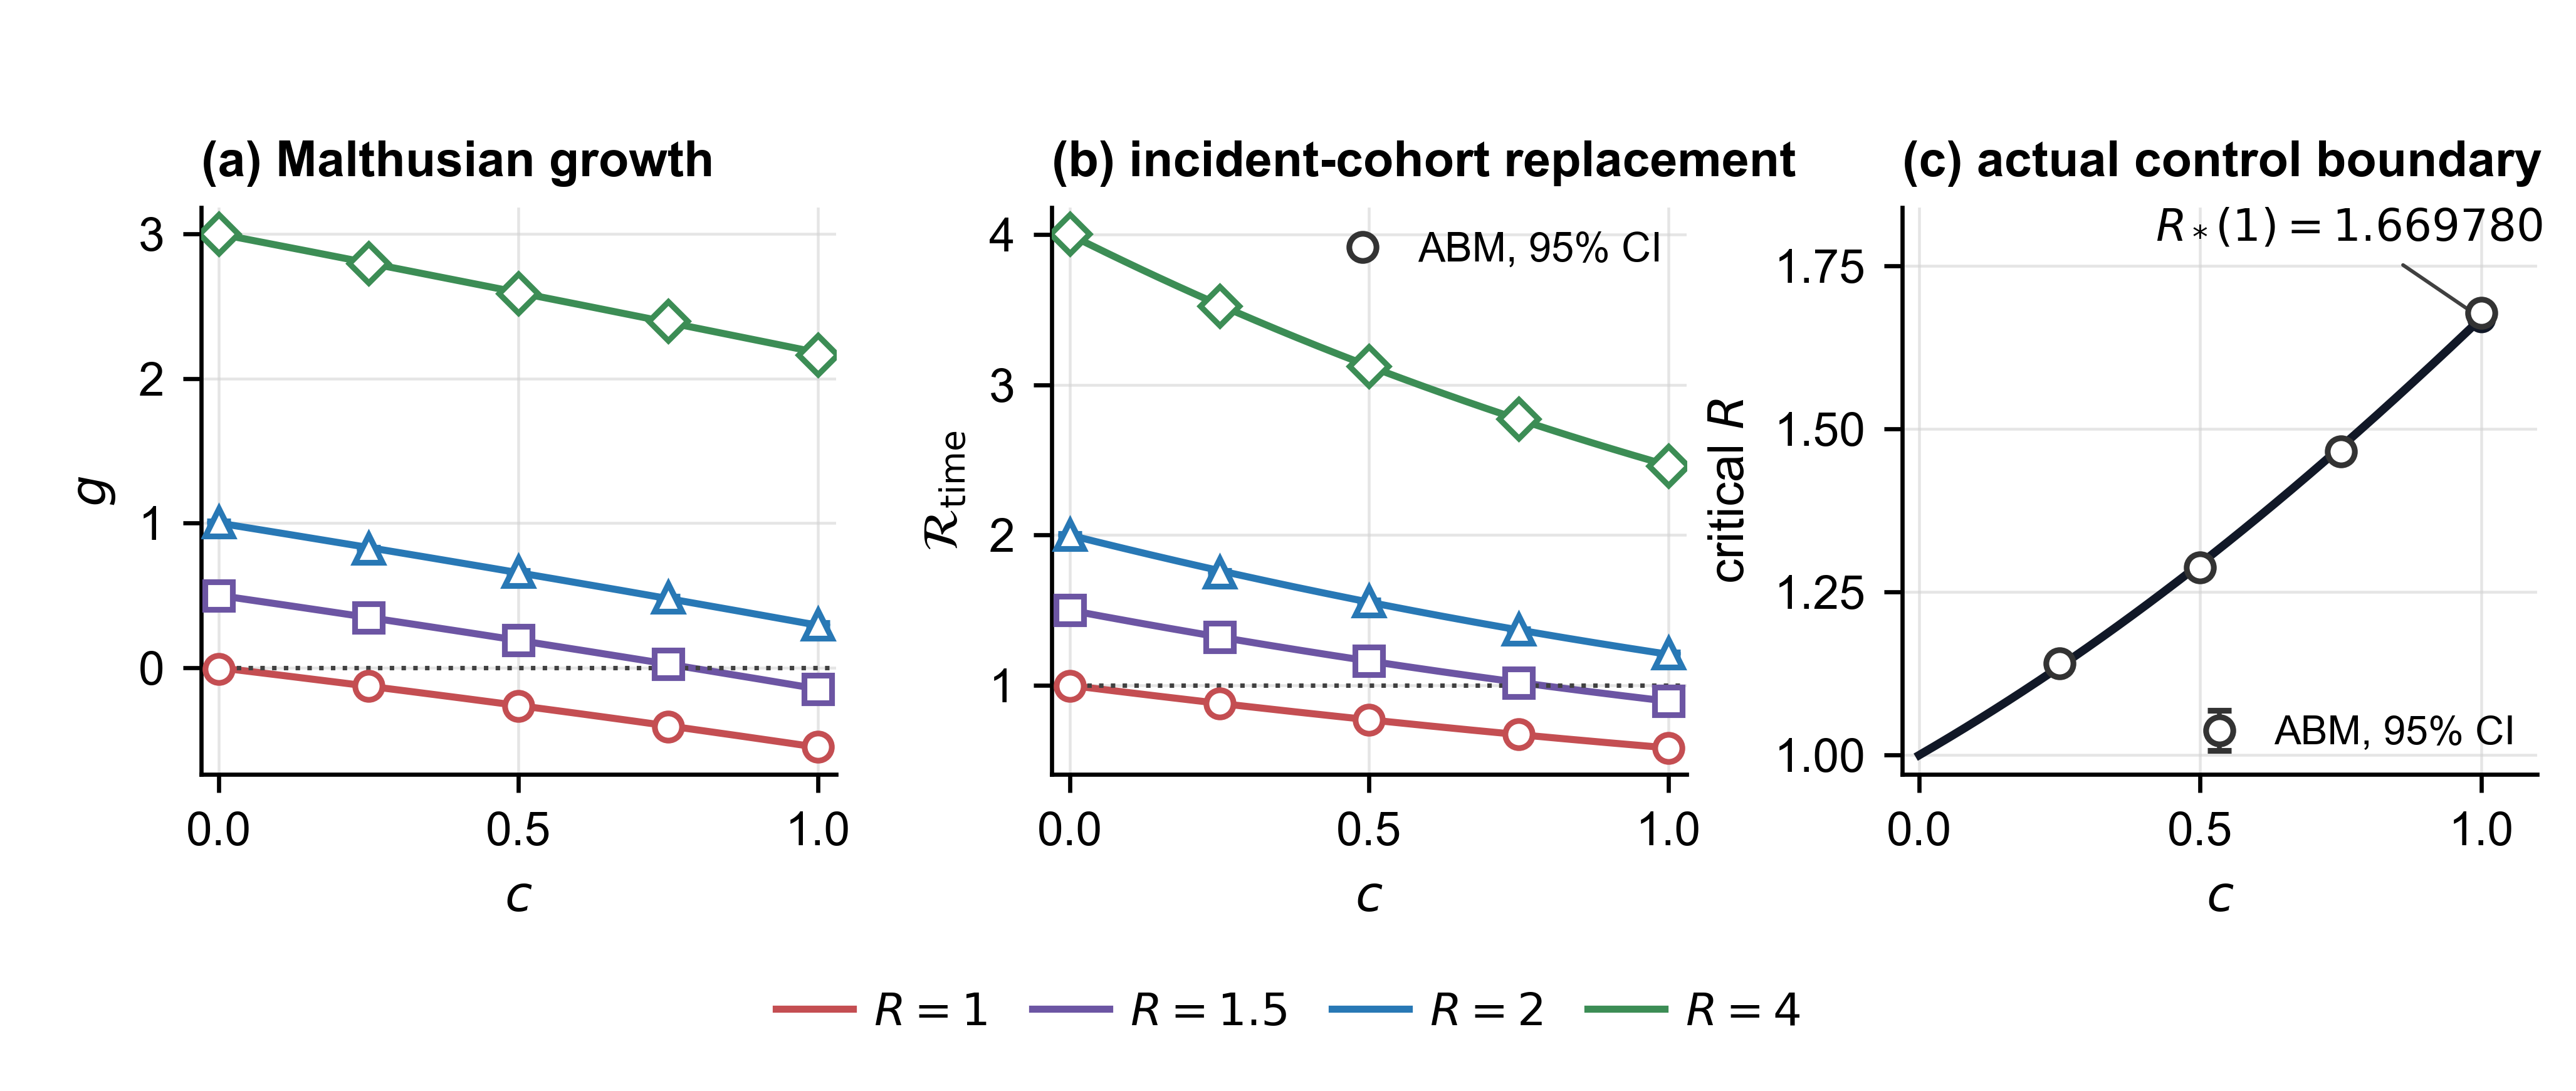
\includegraphics[width=0.99\textwidth]{Fig3.png}
\caption{Malthusian growth, incident-cohort infectious-time replacement, and the actual control boundary under instantaneous one-step forward tracing. \textbf{(a)} Dimensionless Malthusian rate $g(R,c)=R-1-cm_1(R,c)$, with $m_1$ evaluated on the selected QSS branch. Solid curves show the analytical prediction for $R=1,1.5,2,$ and $4$; open symbols show event/person-time estimates from the corresponding constant-pool ABM ensembles, with pointwise 95\% whole-replicate bootstrap intervals. The dotted line marks $g=0$. \textbf{(b)} Incident-cohort infectious-time replacement $\mathcal R_{\mathrm{time}}$, defined as the complete infectious person-time contributed by individuals infected during the cohort-entry window per unit infectious person-time of the infectious population during that window. Solid curves show Eq.~\eqref{eq:6.8}; open symbols show complete-follow-up ABM ensemble estimates. The dotted line marks $\mathcal R_{\mathrm{time}}=1$. \textbf{(c)} Actual selected-QSS control boundary $R_*(c)$, defined by $g(R_*(c),c)=0$. Open circles and intervals show ABM estimates obtained by interpolating between prespecified cells bracketing zero growth. The maximal-regime endpoint is $R_*(1)=1.66978036$. The ABM implements the same event rules as the deterministic hierarchy; the full ensemble protocol and numerical diagnostics are given in Supplementary Material 1, Sections S4.4 and S4.5, respectively.}
\label{fig:fig3}
\end{figure}

\section{Finite-dimensional closures and validation}\label{sec5}

Along complete finite-pool trajectories $R_S(\tau)$ varies with time while the hierarchy remains infinite in depth, so a closure is needed. The question is how much transmission depth must be retained --- and, strikingly, how little suffices.

\subsection{Two closures}\label{subsec5.1}

A depth-$K$ dynamic closure retains $S,I,m_1,\ldots,m_K$ as evolving variables, evolves Eq.~\eqref{eq:2.33} without modification for $1\leq k<K$, and approximates only the first unresolved coordinate $m_{K+1}$. At $c=0$ and fixed $R_S$, the no-tracing recurrence gives the tail ratio $m_{K+1,0}/m_{K,0}=R_S/(R_S+K+1)$; evaluating it at the instantaneous $R_S(\tau)$ defines the local tail map
\begin{equation}
\Phi_{K+1}^{\mathrm{tail}}(R_S;m_K) = \frac{R_S}{R_S+K+1}m_K,
\label{eq:7.2}
\end{equation}
so that the final retained equation is
\begin{equation}
m_K' = R_S(m_{K-1}-m_K) - K m_K + c\left[m_1 m_K - \Phi_{K+1}^{\mathrm{tail}}(R_S;m_K)\right].
\label{eq:7.3}
\end{equation}
Thus $K$ is the deepest genealogical level evolved dynamically, and closure order has a direct mechanistic meaning: it specifies how much transmission depth is retained. During a trajectory with $c>0$ the map is an approximation whose error may reflect both tracing-induced deformation of the tail and dynamical lag as $R_S(\tau)$ changes; it does not assume the evolving genealogy remains on the traced QSS branch. Since $0\leq\Phi_{K+1}^{\mathrm{tail}}\leq m_K$, the supplied coordinate is consistent with the structural bound of Lemma~1, although this does not by itself guarantee that the closed system preserves the full ordering, so admissibility is monitored numerically without state clipping.

The simplest reduction evolves no genealogical coordinate at all. Motivated by the accuracy of Eq.~\eqref{eq:5.4a}, it replaces $m_1$ by its zeroth-order QSS value at the instantaneous transmission strength,
\begin{equation}
\widehat m_1^{(0)}(\tau) = \frac{R_S(\tau)}{R_S(\tau)+1},
\label{eq:7.6}
\end{equation}
reducing the entire system to
\begin{align}
S' &= -R_S I, \label{eq:7.7a}\\
I' &= I\left(R_S - 1 - c\frac{R_S}{R_S+1}\right). \label{eq:7.7b}
\end{align}
Two variables, one algebraic expression, and the mechanistic form of the tracing loss retained. It makes two distinct approximations --- omitting the $c$-dependent deformation of the QSS genealogy, and assuming the genealogy adjusts instantaneously as $R_S$ changes --- which is precisely why it is a useful benchmark: both error sources are identifiable. Since $0\leq\widehat m_1^{(0)}<1$, the supplied coordinate satisfies the counting bound, and the closed system preserves $S\geq0$ and $I\geq0$.

\subsection{Validation against ABM ensembles}\label{subsec5.2}

The closures are assessed at two complementary levels: locally, by comparing the closure-supplied term with the corresponding coordinate measured from the ensemble-mean ABM genealogy at the same observation time, and globally, by comparing the resulting closed trajectory with the ensemble-mean ABM trajectory. Replacing $m_{K+1}$ by any closure function $\Phi_{K+1}$ perturbs only the $m_K$ equation, and by an amount $c[\Phi_{K+1}-m_{K+1}]$ exactly; the transmission, primary-removal, and retained tracing contributions cancel identically. This snapshotwise defect identity and its ensemble estimator are given in Supplementary Material 1, Section S6.1.

Locally, across the 12 $(R,c)$ protocols with $c>0$, the median protocol-level time-mean absolute defect was $0.0472$ for the algebraic QSS closure and $0.0234$, $0.00922$, and $0.00310$ for the depth-1, depth-2, and depth-3 dynamic closures. The local error therefore decreases monotonically with retained depth, and the algebraic closure departs increasingly from local agreement as tracing strengthens, as expected from its two approximations.

Globally, writing $z^C=(S^C/S_0,\,I^C/S_0,\,M_1^C/S_0)$ with $M_1^C=I^Cm_1^C$, the closure trajectory error is
\begin{equation}
E_C = \left[\frac{1}{T}\int_0^T \left\|z^C(\tau)-z^{\ABM}(\tau)\right\|_2^2\,d\tau\right]^{1/2},
\label{eq:7.16}
\end{equation}
reported in Fig.~\ref{fig:fig4} across the tested protocols. The distinction between the two levels matters: local and trajectory accuracy need not order the closures the same way, and most dynamic-closure differences are not resolved from Monte Carlo uncertainty at 120 realizations. Snapshotwise scatter, the depth-$K$ trajectory overlays, and the full protocol tables are given in Supplementary Material 1.

\begin{figure}[htbp]
\centering

\includegraphics[width=0.99\textwidth]{Fig4.pdf}
\caption{Closure-trajectory validation against the ensemble-mean finite-population agent-based model (ABM). The normalized integrated $L^2$ trajectory error $E_C$ in Eq.~\eqref{eq:7.16} is shown against tracing intensity $c$ for (a) the zeroth-order algebraic QSS closure and the dynamic tail closures of depth (b) $K=1$, (c) $K=2$, and (d) $K=3$. The common vertical axis is logarithmic. The compared trajectory vector is $z=(S/S_0,I/S_0,M_1/S_0)$, with $M_1=Im_1$ for each deterministic closure and $M_1$ averaged directly from the raw ABM counts. Points compare each deterministic closure with the 120-realization sample ensemble-mean ABM trajectory. Error bars are 95\% Monte Carlo intervals obtained by applying a first-order delta method to complete-realization influence values; they quantify uncertainty in the estimated ensemble mean rather than replicate-to-replicate trajectory spread. Downward arrowheads at the lower plotting boundary indicate intervals that reach zero, which cannot be displayed on the common logarithmic axis. Colors and markers denote $R=1$ (coral circles), $R=1.5$ (purple squares), $R=2$ (blue triangles), and $R=4$ (green diamonds); all curves are solid. Simulations use $S_0=8000$, $I_0=160$, $c\in\{0,0.25,0.5,0.75,1\}$, 120 independent realizations per $(R,c)$ cell, and 151 observation times on $0\leq\tau\leq5$; tracing is activated at $\tau=0.5$. The integral includes the preactivation interval $0\leq\tau<0.5$ and therefore includes initial genealogical adjustment, particularly for the algebraic QSS closure. Smaller values indicate closer agreement with the sampled ensemble-mean event-level process; most dynamic-closure differences are not resolved from Monte Carlo uncertainty at 120 realizations.}
\label{fig:fig4}
\end{figure}

Figure~\ref{fig:fig5} shows representative finite-pool trajectories at $R=4$ for the zeroth-order algebraic QSS closure against the corresponding ensemble-mean ABM trajectories, complementing the integrated errors by showing the timing and direction of the discrepancies after tracing activation. The algebraic closure assigns $m_1$ instantaneously from $\widehat m_1^{(0)}(\tau)$ and therefore represents neither tracing-induced deformation nor genealogical memory; the dynamic closures, which retain genealogical variables explicitly, do represent their finite-time relaxation as $R_S(\tau)$ changes, and their overlays are given in Supplementary Material 1. That a two-variable algebraic reduction tracks the susceptible and infectious trajectories as closely as it does is the practical payoff of the construction: the genealogy enters the population equations through a single term $cm_1I$, and a one-line approximation of $m_1$ already captures most of it.

\begin{figure}[htbp]
\centering
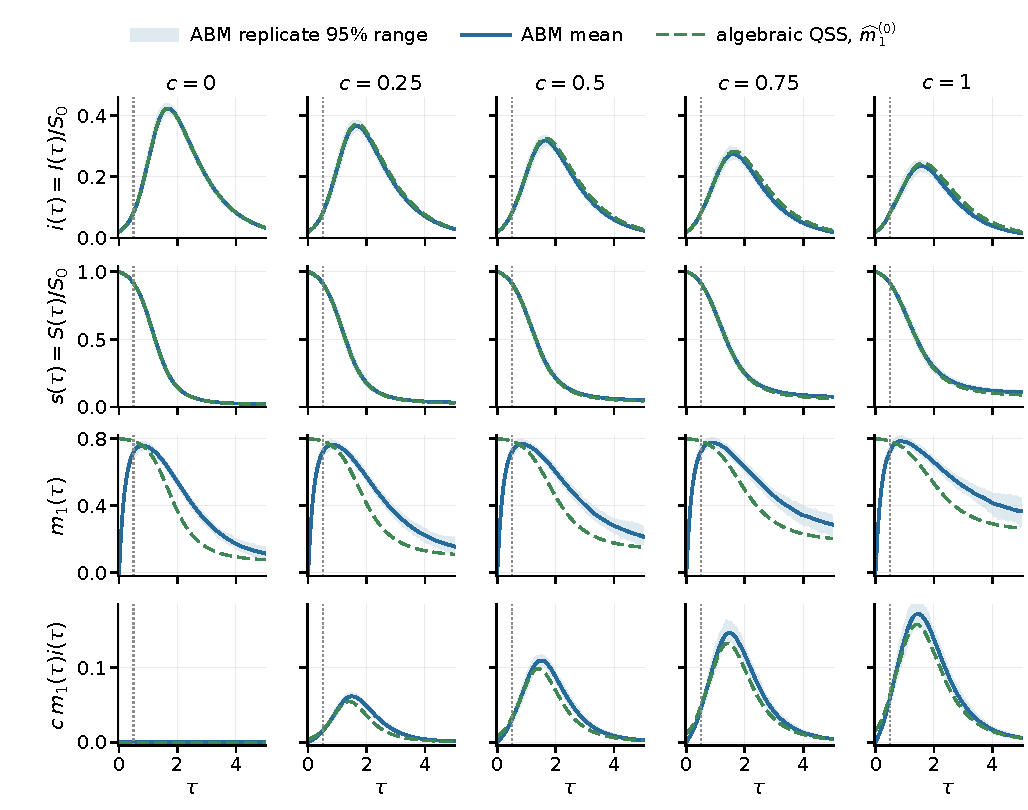
\includegraphics[width=0.99\textwidth]{Fig5.pdf}
\caption{Representative finite-pool trajectories for the zeroth-order algebraic QSS closure at $R=4$. Columns show $c=0,0.25,0.5,0.75$, and $1$; rows show $i=I/S_0$, $s=S/S_0$, $m_1=M_1/I$, and the normalized deterministic tracing flux $c\,m_1(\tau)i(\tau)$. Blue curves are the sample ensemble-mean ABM trajectory and pale bands are pointwise 2.5th--97.5th replicate percentiles across 120 independent realizations. The green dashed curve is the algebraic closure $\widehat m_1^{(0)}(R_S)=R_S/(R_S+1)$ (Eq.~\eqref{eq:7.6}), which assigns $m_1$ instantaneously from the susceptibility-adjusted transmission strength $R_S(\tau)$ and does not retain tracing-induced genealogical memory. The vertical dotted line marks activation of forward tracing at $\tau=0.5$. Simulations use $S_0=8000$, $I_0=160$, and 151 observation times on $0\leq\tau\leq5$, with $(\gamma/\Gamma,\gamma_c/\Gamma,p_f)=(0,1,c)$. The trajectories shown are the same $R=4$ ABM ensemble underlying the $E_C$ errors reported in Fig.~\ref{fig:fig4}.}
\label{fig:fig5}
\end{figure}

\section{Discussion}\label{sec6}

The contribution of this work is a particular choice of aggregation coordinates. Individuals contribute through their positions relative to local roots and are grouped by descendant depth, which preserves the directional information on which tracing acts while keeping the resulting population variables directly interpretable. It thereby provides a systematic link between tracing rules defined through infector--infectee relationships and the terms through which those rules enter population-level epidemic equations.

The benefit of this coordinate is that it remains both interpretable and structurally simple. Each $M_k$ counts a tangible feature of the active genealogy: root--descendant relationships at depth $k$. The first moment gives the forward-tracing burden directly, while each deeper moment appears for a clear reason --- it supplies the information needed to evolve the preceding one. In the present one-step model the hierarchy is infinite but nearest-neighbor in transmission depth, with every new level introducing only the next required depth. Normalizing by the infectious population then separates epidemic magnitude from genealogical shape, so that relaxation of the root-relative structure can be studied independently of whether prevalence is growing or declining, and the quasi-steady approximation reduces the normalized hierarchy to a scalar relation with equivalent continued-fraction and modified-Bessel representations while retaining the influence of all descendant depths.

The hierarchy also shows why no single transmission depth is sufficient for every epidemiological quantity. The incident-cohort measure $\mathcal R_{\mathrm{time}}$, defined for an individual sampled at infection, depends on its active-ancestor chain, and in the present scaling
\begin{equation}
\mathcal R_{\mathrm{time}} = R(1-c/2) + O(c^2).
\label{eq:8.1}
\end{equation}
After matching parameters and sampling convention, this agrees at first order with earlier forward-tracing results obtained from infectious-age and branching-process formulations \cite{muller2016,okolie2020}. The root-centered population formulation therefore recovers a result previously derived through individual-level approaches.

The control boundary should not be mistaken for the limit of the intervention's epidemiological effect. Maximal one-step tracing reverses early growth only when $R<R_*(1)\approx1.67$. Above this boundary tracing does not make the epidemic subcritical, but across the supercritical regimes examined it still reduces the future infectious activity generated by newly infected cases by approximately 40\%. One-step forward tracing can therefore markedly reduce future infectious activity even when it does not achieve control.

The framework sits alongside branching-tree, pairwise-moment, and component-size hierarchies, but closure occurs along a different coordinate. Branching-tree models retain genealogical relationships in the early-growth limit, pairwise models retain local network configurations, component-size models retain the size or composition of traced components, and the present framework retains descendant depth relative to overlapping roots \cite{muller2000,taylor2012,sharkey2015b,zhang2022}. Closure order therefore has a direct mechanistic meaning: it specifies how much transmission depth is retained. Over the regimes examined, low-order closures reproduce both the transient genealogical structure and the principal population trajectories, and the zeroth-order algebraic closure $\widehat m_1^{(0)}(R_S)=R_S/(R_S+1)$ captures the susceptible and infectious trajectories comparatively well.

The quantitative results are conditional on a well-mixed SIR-type epidemic with one recorded infector per infection, immediate infectiousness, exponentially distributed primary-removal times, instantaneous tracing of active direct infectees, independent tracing decisions, complete ascertainment of detected cases, and no repeated tracing cascade. These assumptions define the scope of the calculated control boundary, the reduction in future infectious activity, and the closure results, and they provide a transparent setting in which the construction can be developed in full, from individual tracing events to population equations, early-growth analysis, and finite-depth closure. Contact heterogeneity, network clustering, and tracing delays can materially alter tracing dynamics and control conditions \cite{house2010,muller2016,kretzschmar2020}. The numerical values obtained here should therefore not be interpreted as protocol-independent limits or as empirical estimates of the effectiveness of operational tracing programs.

Extensions to other tracing protocols and disease histories would begin by identifying the root-relative positions that determine the intervention's immediate action and the additional positions needed to evolve those quantities after the event, then aggregating these positions across active roots to generate the corresponding population hierarchy before closure is imposed. Backward tracing would introduce active-ancestor and collateral-branch coordinates, while bidirectional tracing would couple ancestor and descendant coordinates; existing studies show both the potential value of these strategies and the dependence of their relative performance on network structure and disease dynamics \cite{bradshaw2021,kojaku2021,juul2023}. Repeated tracing would require additional coupled coordinates, latent periods would produce stage-specific or multitype hierarchies, and explicit delays would add infection-age or tracing-age structure \cite{muller2016,kretzschmar2020}. Not every such extension will preserve the nearest-neighbor recurrence; some may produce multitype, multi-index, or age-structured systems. The underlying questions, however, remain the same: which parts of transmission history determine the intervention, what further information is required to evolve its population-level effect, and which reduction provides an appropriate balance between mechanistic detail and tractability?

\section*{Supplementary material}

The supplementary material consists of the following four files. Labels and
filenames are used consistently throughout the manuscript and the supplements.

\textit{Supplementary Material 1 (supplementary\_material\_1.pdf).} Model
construction details, analytical and numerical details for the quasi-steady
solution, the perturbative construction, technical results and the
large-population ensemble protocol, the finite-population agent-based benchmark,
closure validation, and reproducibility files (Sections S1--S7, Tables
S1--S10, Figs.~S1--S8).

\textit{Supplementary Material 2 (supplementary\_material\_2.xlsx).} All 780
dimensional parameterizations, published trajectory-error and convergence
summaries, and deterministic-reference and event-term checks.

\textit{Supplementary Material 3 (supplementary\_material\_3.zip).} Available
executable and audit code, numerical tables and data, event-term data,
figure-generation files, software requirements, and reproducibility
documentation.

The code and archives cited in Sections S2.3 and S7 are supplied in
Supplementary Material~3.

\section*{CRediT authorship contribution statement}

\textbf{Seyfullah Enes Kotil:} Conceptualization, Methodology, Software,
Formal analysis, Validation, Investigation, Visualization, Writing -- original
draft, Writing -- review and editing.

\section*{Declaration of competing interest}

The author declares that they have no known competing financial interests or
personal relationships that could have appeared to influence the work reported
in this paper.

\section*{Funding}

This research did not receive any specific grant from funding agencies in the
public, commercial, or not-for-profit sectors.

\section*{Data availability}

All data generated or analyzed during this study are included in this article,
in its supplementary material (in particular Supplementary Materials 2 and 3),
and in the accompanying repository at
\url{https://github.com/kotilboun/Overlapping_roots}. The code supporting the
findings of this study is supplied in Supplementary Material 3 and is available
at the same repository.

\section*{Acknowledgements}

The author thanks Huseyin Tunc and Esra Ozge Asan for valuable discussions.

\section*{Declaration of generative AI and AI-assisted technologies in the manuscript preparation process}

During the preparation of this work the author used ChatGPT (Sol 5.6, OpenAI)
and Claude Code (Anthropic) in order to assist with document organization,
language editing, code generation, figure-generation workflows, and
proofreading. After using these tools, the author reviewed and edited the
content as needed and takes full responsibility for the content of the
published article.

\bibliographystyle{elsarticle-num}
\bibliography{references}

\end{document}
